\startchapter{Discussion, Platform and Results}
\label{chapter:eval}
\section{Introduction}
In this chapter we present a full description of the automated tool. The provision of a machine which executes the methodologies previously described concretes their definition and propels them towards acceptance as standard practice. Interested parties can use this tool as a source of reference when describing their own investigations. The HTS further allows the collection and centralization of data. The avid use of this tool in the hardware security science community will naturally create a catalog of information from which statistical analysis on the field can be performed.  
\section{Web Environment}
The HTS is comprised of three applications which perform the analysis of the quantitative methods described in the previous chapter in sections \ref{section:Classification}, \ref{section:Detection} and \ref{section:Attacks}. The applications are nested in a web site that is easily accessible worldwide, provides documentation and instructions for users as well as an easy to navigate user interface. The system operates primarily on an application server which performs all of the computation and generates page mark-up to minimize overburdening client-side browsers with processing responsibility. The server communicates directly with a remote database used to store user login and account information, application data (attributes, categories and the computation matrices) as well as any work performed by the user both complete or incomplete. Both the application server and the database are hosted on \textit{Microsoft's Azure Cloud} platform. The cloud platform improves reliability, portability and flexibility, provides 'on-demand' resources that are automatically managed for scalability requirements and provides the ability for maintenance to take place anywhere.
\subsection{Technologies Used}
In this section we provide a review of the tools and technologies used to implement the HTS. 
\subsubsection{ASP.NET Web Form Framework}
The web application is built using \textit{Microsoft's} ASP.NET web application framework \cite{ASP} which provides multiple programming models for advanced web application development. The trojan classification tool employs .NET's  \textit{Web Forms} model. The \textit{Web Forms} model provides pages that are requested by a client-side browser. The server uses what is referred to as \textit{"behind the page"} code to dynamically compile application logic and generate HTML markup which is sent to the client. The use of this technology provides automated compatibility with any browser, powerful C\# application logic programming capability, intuitive inter-end state management and easy scalability.
\subsubsection{Entity Framework}
Entity Framework \cite{Entity} is an object-relational mapper designed for the .NET framework. It allows for easy database schema and query design. Use of Entity allows server developers to model database entities and table relationships using a high-level programming layer which is easy to integrate into application logic. Entity also provides model visualizers for powerful database design. To demonstrate, Entity's visualizer was used to create Figure~\ref{fig:DBModel}. Entity was used to design the database and application specific queries used regularly in the application.

\begin{figure}
	\centering
	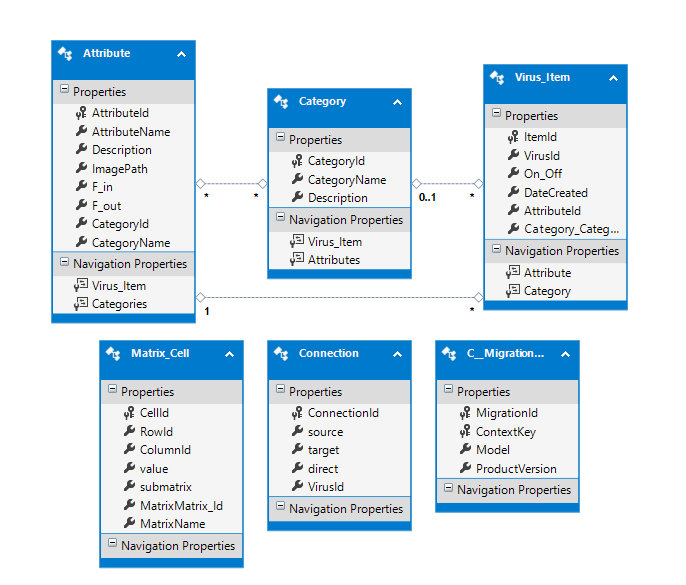
\includegraphics[width=1\linewidth]{figures/DBModel}
	\caption[Visual Representation of the Database Design]{Visual Representation of the Database Design}
	\label{fig:DBModel}
\end{figure}
\subsubsection{Data Driven Documents (D3)}
\textit{Data-Driven Documents (D3)} \cite{D3} is a JavaScript library for manipulating documents based on data. The results of the server side virus description are parsed into a JSON string which is received by the client side browser. The client side JavaScript employs the D3 library to create a visualization representing the received attributes as nodes and their interconnections as directed arrows.  
\subsubsection{Microsoft Azure}
\textit{Microsoft's Azure} cloud system is a high performance distributed hosting platform used to host both the database and application server for the HTS. The platform was built to allow developers the ability to design, host and manage applications using a variety of technologies. The powerful yet flexible infrastructure provides a reliable and responsive host for the system.
\begin{figure}
	\centering
	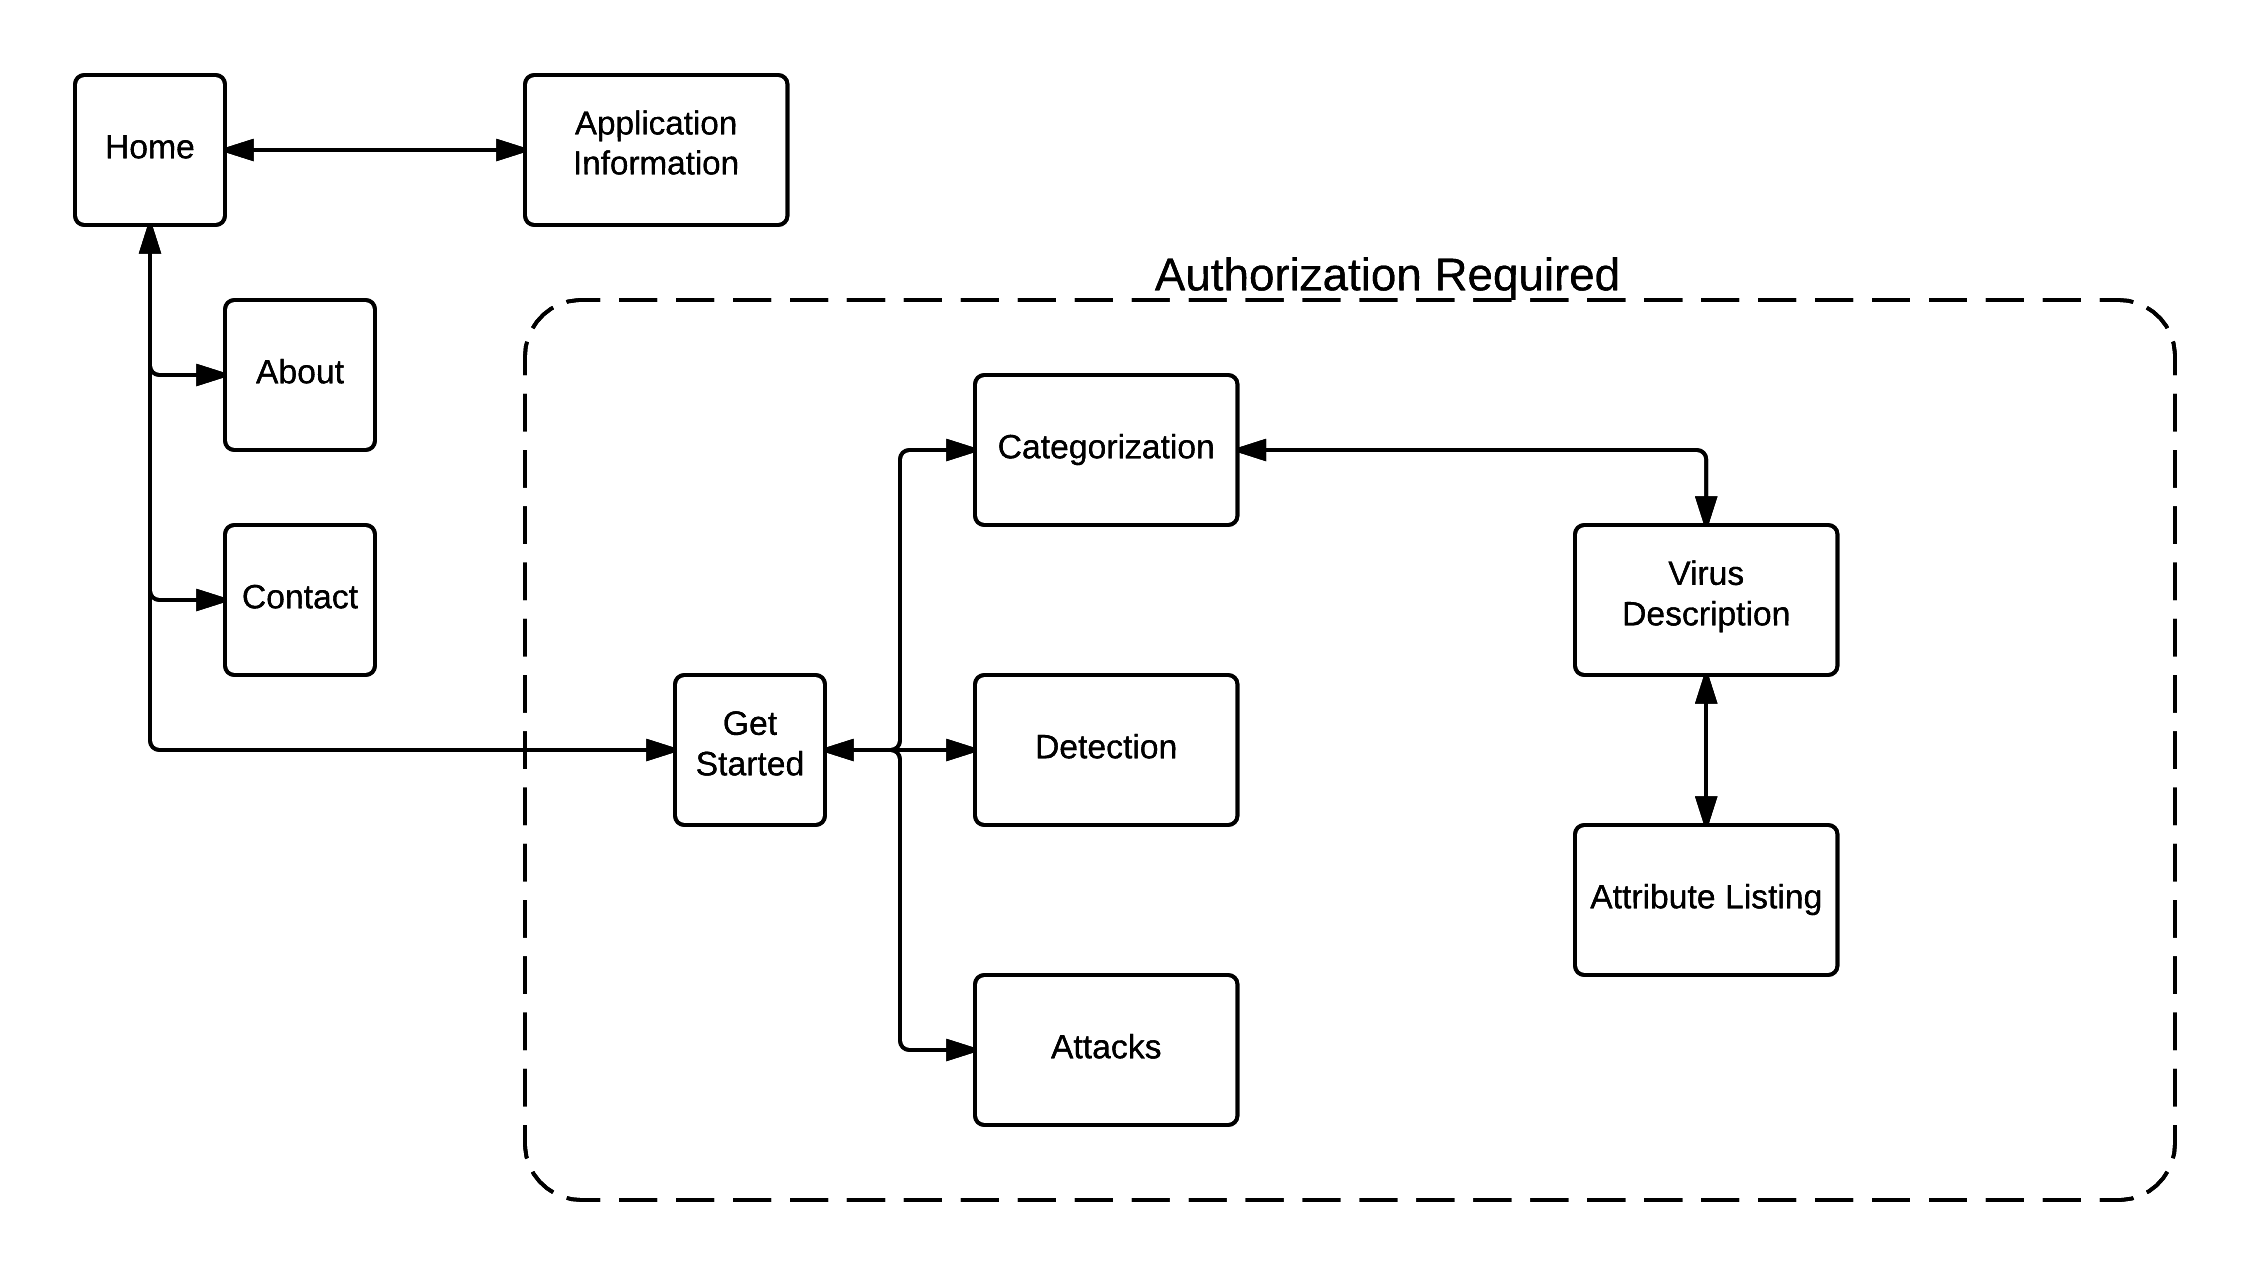
\includegraphics[width=1\linewidth]{figures/WebsiteArchitecture}
	\caption[Overview of Web Site Architecture]{Overview of Web Site Architecture}
	\label{fig:WebsiteArchitecture}
\end{figure}
\subsection{Website Architecture}
Figure~\ref{fig:WebsiteArchitecture} provides a simple diagrammatic overview of the structure of the trojan system website. The \textit{home, contact} and \textit{about} pages are accessible to all traffic as well as the application information page which consists of three separate pages all providing background information for each of the primary applications. Users are required to create an account and be logged in to access the remainder of the site as displayed by the dashed line of Figure~\ref{fig:WebsiteArchitecture}. Email confirmation is used to verify user account applications. 

Once users are authorized they are granted access to the \textit{Get Started} page which provides basic information and access to each of the applications. To perform the classification method outlined in section \ref{Classification} users are required to browse through a listing of the available 33 attributes shown in Figure~\ref{fig:HW_trojan}. The selected attributes are then displayed on the \textit{Virus Description} page where the user is able to visualize the result. For a more complete description of this application refer to section \ref{CatApp}.

\subsection{Distributed System Architecture} \label{Architecture}
As previously mentioned the hardware trojan system is hosted and operated in the 'cloud'. Microsoft provides a cheap and powerful cloud service named \textit{Azure} which is discussed in section \ref{AzureDesc}. The \textit{Azure} system is comprised of multiple server nodes and the HTS is hosted primarily in the western US node in California. 
\begin{figure}
	\centering
	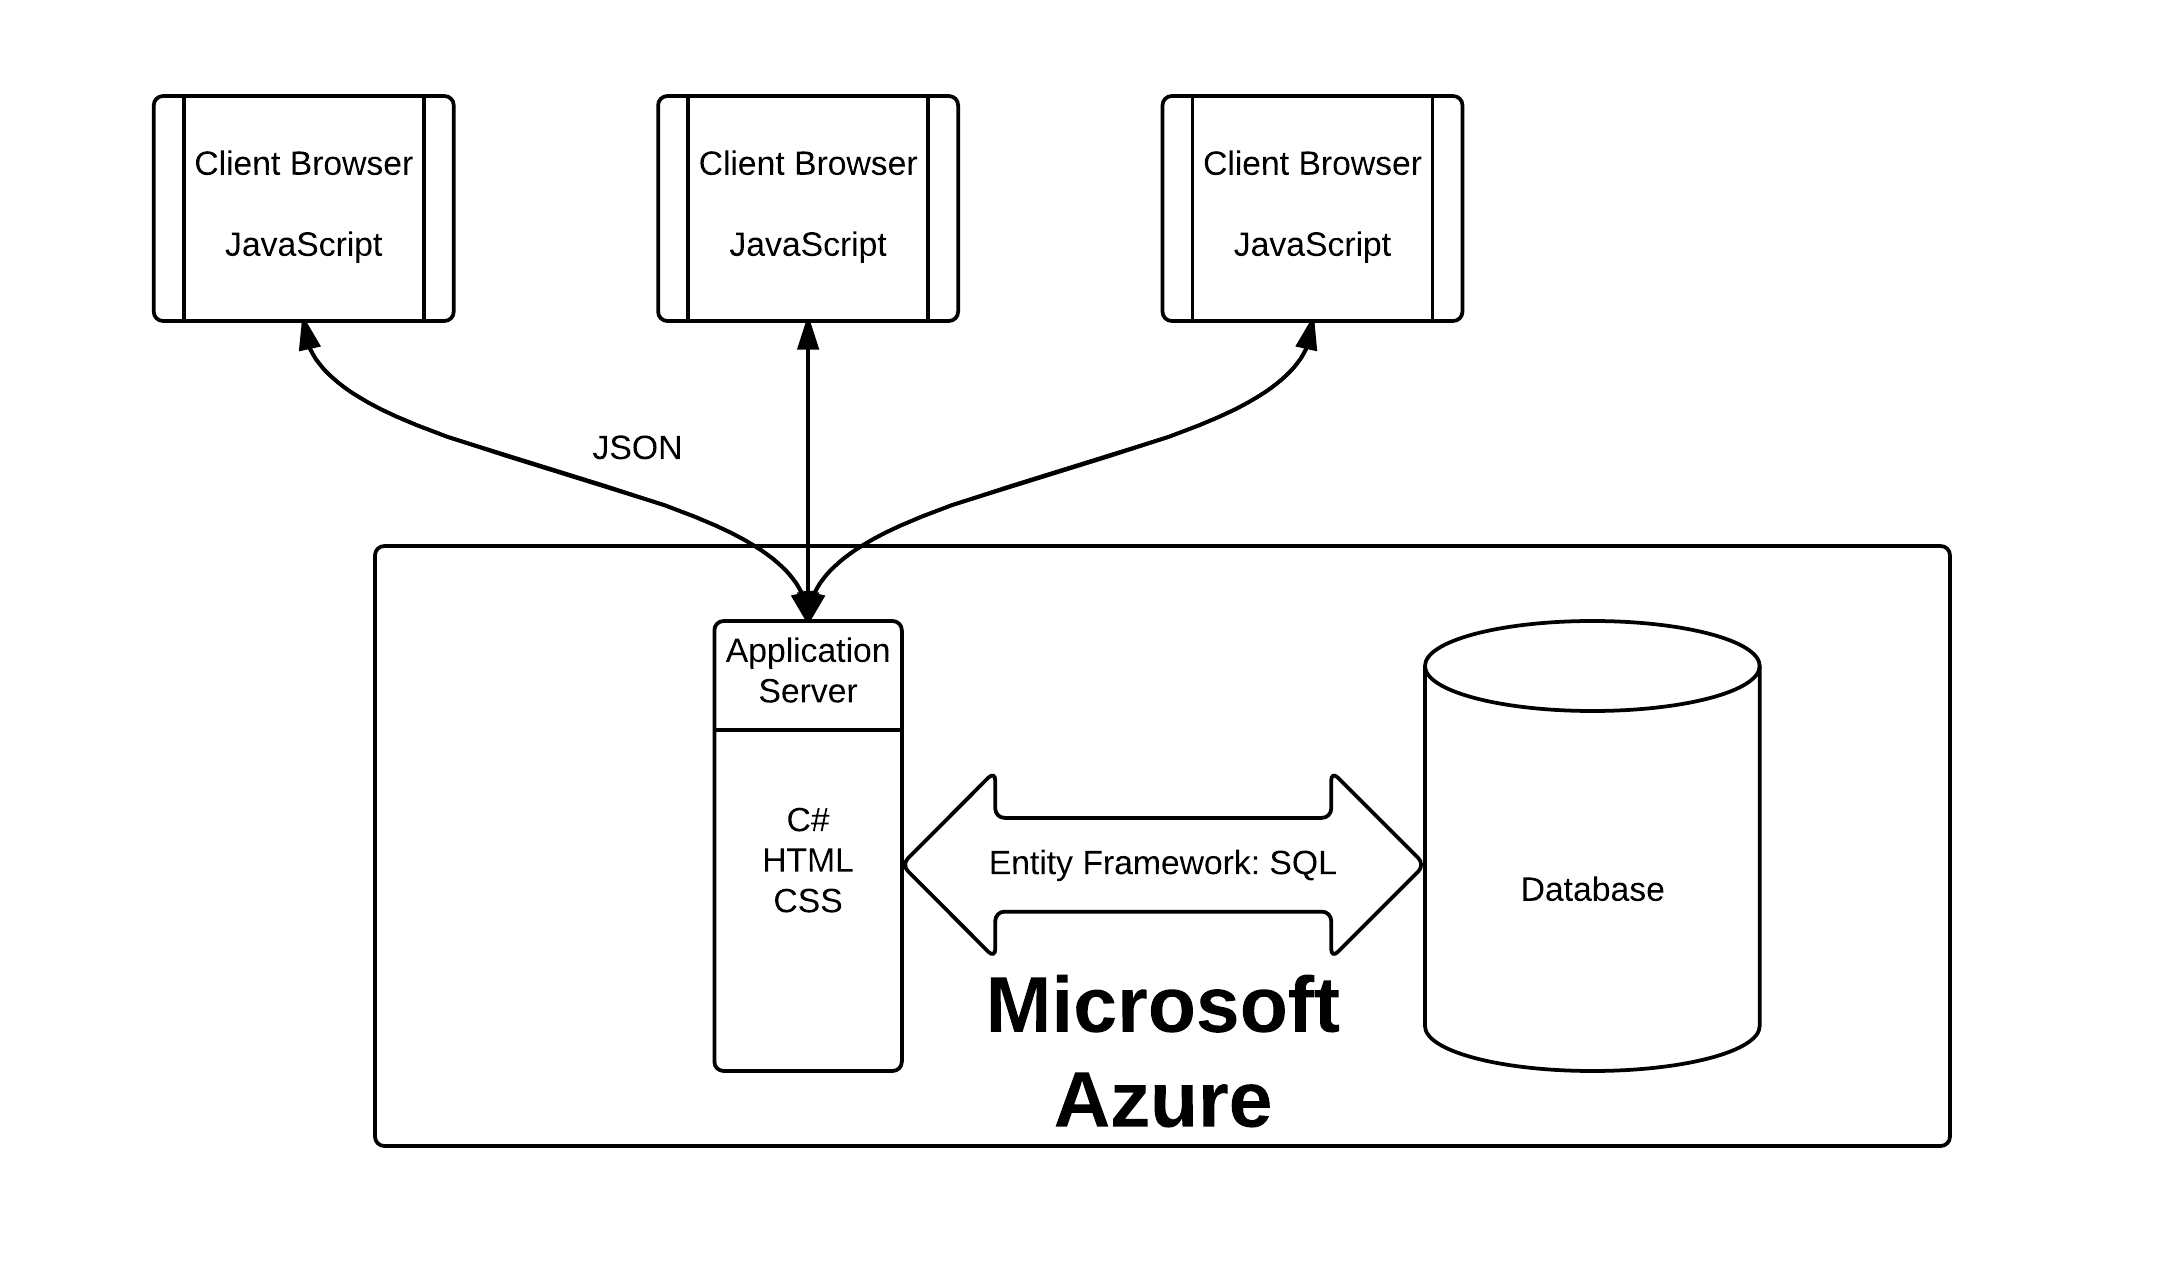
\includegraphics[width=0.9\linewidth]{figures/TrojanDistribution}
	\caption[Distribution of Trojan System]{Distribution of Trojan System}
	\label{fig:TrojanDistribution}
\end{figure}
The application server and the database, both in the 'cloud', are assigned network resources as needed. This dynamic allocation reduces service fees and provides a well defined structure for scalability. In addition Azure provides by the minute statistics for site management including traffic and data routing, data usage, page view statistics and site access locations as show in Figure~\ref{fig:azureReport}.
\begin{figure}
	\centering
	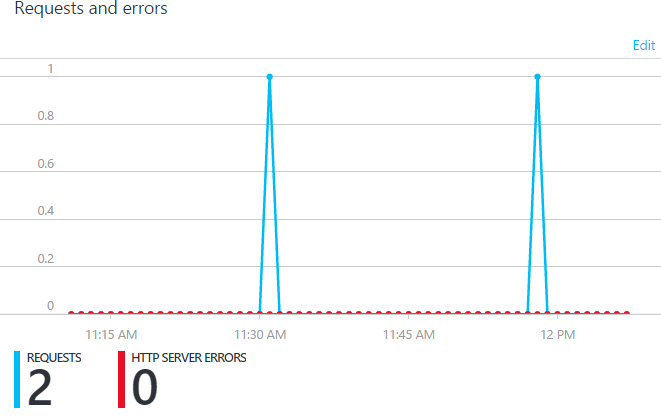
\includegraphics[width=.9\linewidth]{figures/azureReport}
	\caption[Example of Website Access and Error Statistics]{Example of Website Access and Error Statistics}
	\label{fig:azureReport}
\end{figure}
\section{Applications}
\subsection{Classification} \label{Application:Classification}
The trojan classification tool is built on an on-line store model. A list of available attributes is provided for users to select from in a check box style. Figure~\ref{fig:attributeList} is a screen shot of the attribute selection page. By selecting one of the four buttons lining the header of the screen the attribute list page can be filtered to a particular category; in the case of Figure~\ref{fig:attributeList} the page has been filtered to only display attributes of the \textit{Abstraction} category. Figure~\ref{fig:DBModel} is a visual representation of the schema used in the database. Note how the \textit{Attribute} and \textit{Category} entities hold a one to many relationship. When one of the filter buttons in Figure~\ref{fig:attributeList} is selected the corresponding \textit{Category} entity is selected from the database and its \textit{Attributes} navigation key is used to find all related entries in the \textit{Attributes} table. The result is then displayed on the page.\newline
\begin{figure}
	\centering
	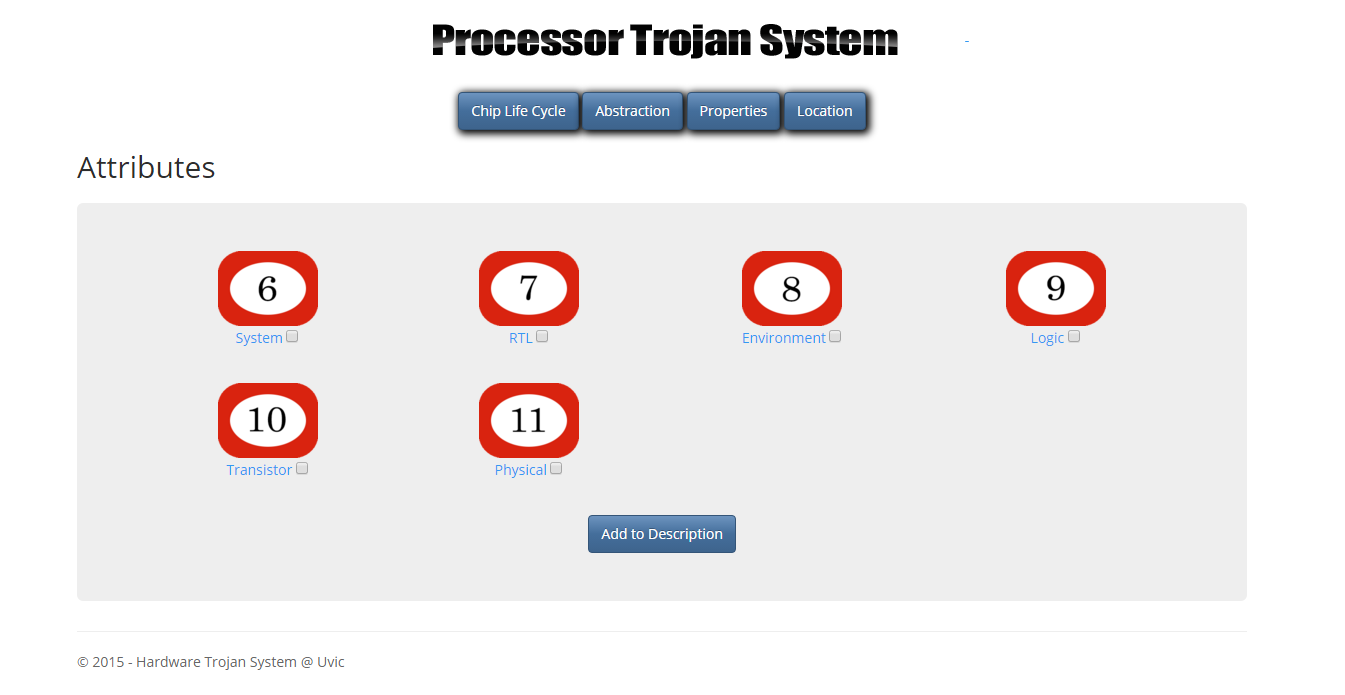
\includegraphics[width=.95\linewidth]{figures/attributeList}
	\caption[The Attribute Selection Page Filtered for Abstraction]{The Attribute Selection Page Filtered for Abstraction}
	\label{fig:attributeList}
\end{figure}

When the user makes a selection of attributes and selects the 'Add to Description' button the selected attributes are added to a 'Shopping Cart' which is assigned a unique id based on the Http session state. This 'Cart' is then stored in the database as a list of objects in the \textit{VirusItems} table which includes the user's unique id string and the id string for the cart. When the user is finished making selections they are transferred to the 'Virus Description' page which can be seen in Figure~\ref{fig:VirusDescription}. The 'Virus Description' page queries the database for the current 'Shopping Cart' by searcing the \textit{VirusItems} table for all entries that match the current users id key and the current session state key.\newline

Each entry in the cart contains an 'On/Off' value that allows the user to add the item to 'Virus Description' page then easily toggle each on and off. The provided grid displays the pertinent information for each entry in the cart as well as the 'On/Off' toggle and the ability to remove a chosen item from the cart.\newline
\begin{figure}[h]
	\centering
	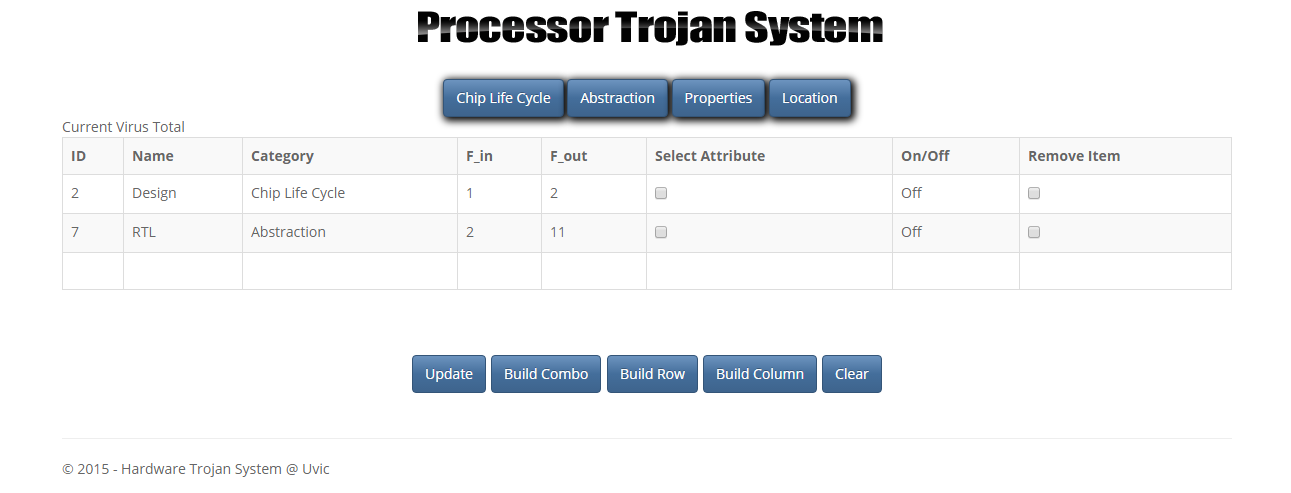
\includegraphics[width=1.1\linewidth]{figures/VirusDescription}
	\caption[The Virus Description Page]{The Virus Description Page}
	\label{fig:VirusDescription}
\end{figure}
\begin{figure}
	\centering
	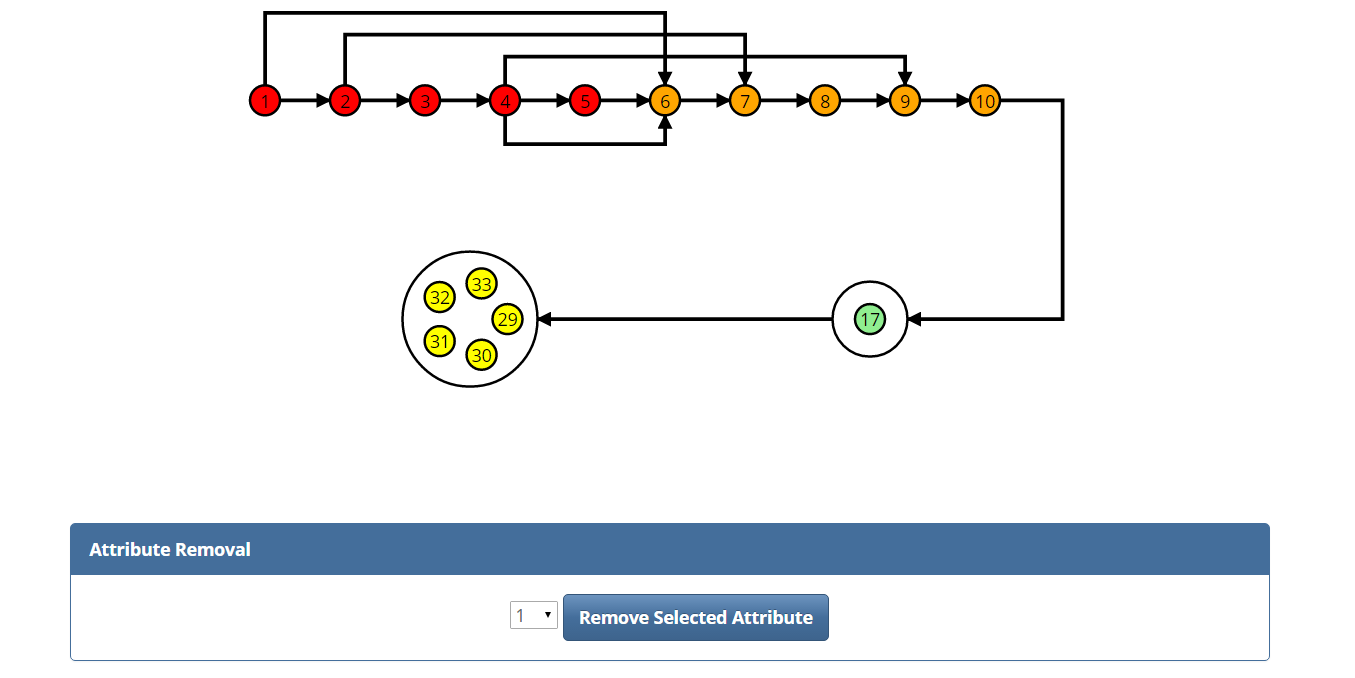
\includegraphics[width=1\linewidth]{figures/visualization}
	\caption[A Visual Representation of a Trojan Virus]{A Visual Representation of a Trojan Virus}
	\label{fig:visualize2Screen}
\end{figure}
\begin{figure}
	\centering
	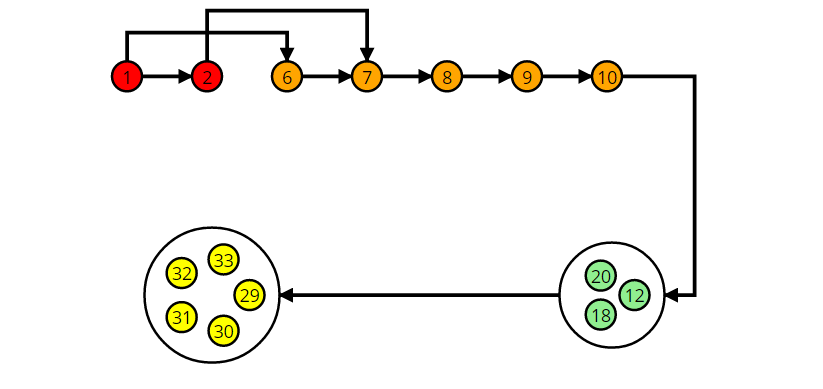
\includegraphics[width=0.9\linewidth]{figures/visualizationRemoved}
	\caption[The Visual Representation after Attribute 4 is Removed]{The Visual Representation after Attribute 4 is Removed}
	\label{fig:visualizationRemoved}
\end{figure}

When the user has finished their attribute selections and toggled all of the needed attributes to 'On' via the 'Update' button they are able to use the 'Build Combo' button. The HTS performs the matrix analysis described in section \ref{section:Classification} and uses the D3 JavaScript API \cite{D3} to draw the directed graph shown in Figure~\ref{fig:visualize2Screen}.\newline

As can be seen in Figure~\ref{fig:visualize2Screen} the classification tool provides a drop down list that allows the user to make modifications to the produced graph. To investigate scenarios of trusted insertion points or undesired attributes the user is able to remove attibutes from the visualization. Figure~\ref{fig:visualizationRemoved} demonstrates the resulting visualization after attribute 4 has been removed from the graph of Figure~\ref{fig:visualize2Screen}. When an attribute is removed the system performs a modified version of the \textit{Bellman-Ford Shortest Path} algorithm developed specifically for this application.\newline

Finally, the classification tool computes and provides the severity rating for the computed trojan according to the method described in section \ref{section:Detection}, as can be seen in Figure~\ref{fig:severityRatin}. Once the user is satisfied with the resulting trojan they have built they can save their work via the 'Save' button at the bottom of the page which is not shown and include a 'nickName'. The virus and corresponding severity rating are saved in the database for access by the detection application described in section \ref{Application:Detection}.

\begin{figure}[h]
	\centering
	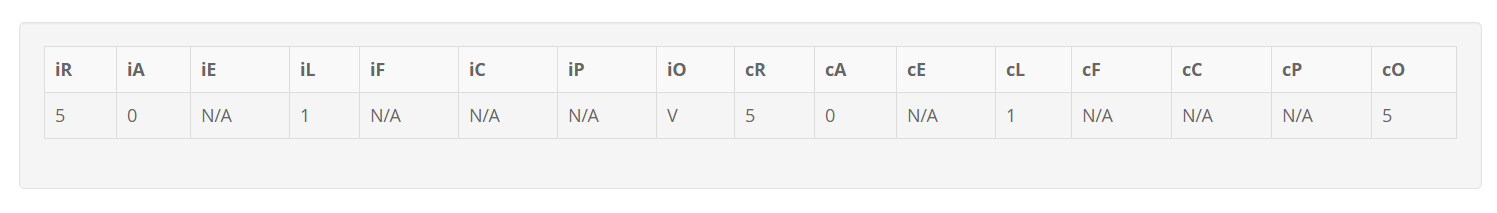
\includegraphics[width=1\linewidth]{figures/severityRatin}
	\caption[The Calculated Severity]{The Calculated Severity}
	\label{fig:severityRatin}
\end{figure}
\subsection{Detection} \label{Application:Detection}
When developers produce a new method of detecting hardware trojans they require some means of determining how it compares to currently known viruses and other detection methods. The ranking system described in section~\ref{Review} provides a means for these methods to be compared and contrasted. In the HTS \textit{Detection} application developers are able to investigate their methods systematically and derive a quantitative status value. Figure~\ref{fig:newDetection} provides a screen shot of the user interface used to create a coverage vector for a new detection method. The user is able to select values for each of the eight classes as well as assign the method a name. When saved this vector is stored in the database, related to the user's account. 
\begin{figure*}
	\centering
	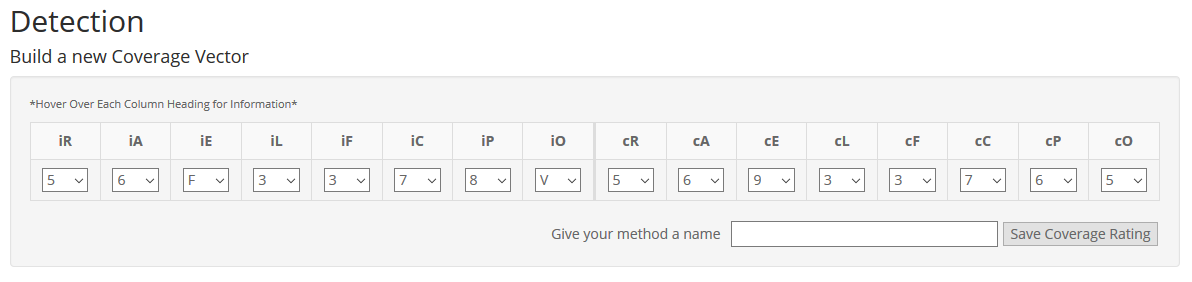
\includegraphics[width=.9\linewidth]{figures/newDetection}
	\caption[The User Interface for Creation of a new Coverage Vector for a Detection Method]{The User Interface for Creation of a new Coverage Vector for a Detection Method}
	\label{fig:newDetection}
\end{figure*}
\begin{figure*}
	\centering
	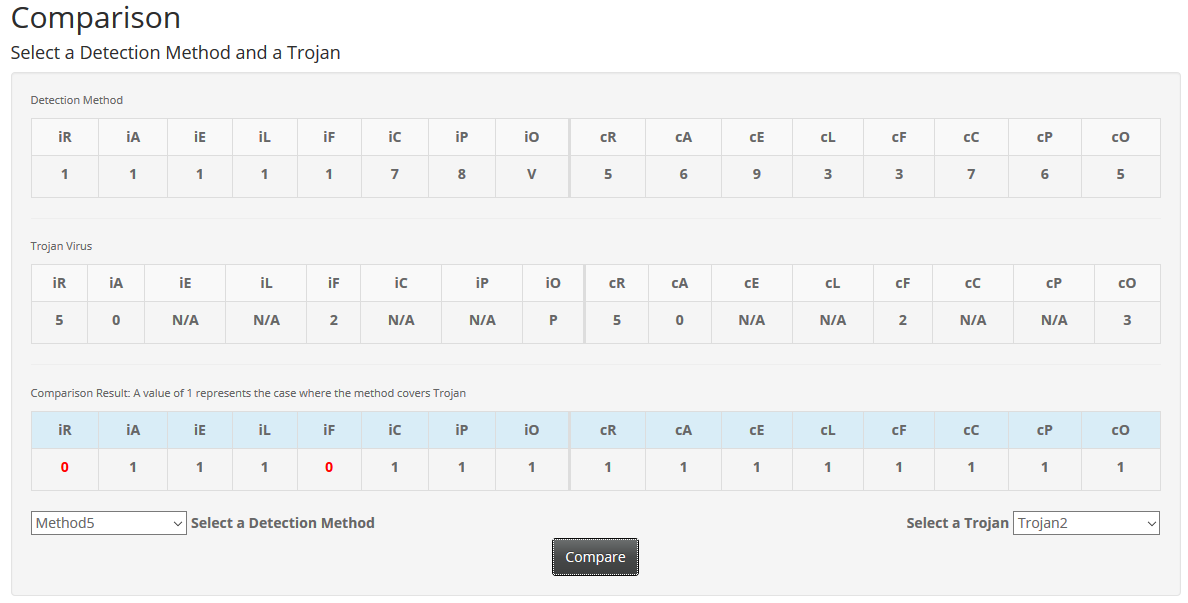
\includegraphics[width=0.9\linewidth]{figures/comparison}
	\caption[Comparison of a Detection's Coverage Vector and a Trojan's Severity Vector]{Comparison of a Detection's Coverage Vector and a Trojan's Severity Vector}
	\label{fig:comparison}
\end{figure*}
The HTS provides a number of automated tools that allow for the analysis of trojan viruses and detection methods. One such tool is the Trojan classification system described in \cite{meCategorization} which employs a method of visualizing the categorization scheme described in \cite{SamerCategorization}. The classification tool described in \cite{meCategorization} provides and additional feature which constructs a severity rating for any trojan analyzed. These ratings can be saved to the database to be used in the detection tool. Please refer to \cite{meCategorization} for more information. In the detection application users are able to search their saved viruses and retrieve the severity ratings to use for comparison. In Figure~\ref{fig:comparison} it can be seen how the comparison tool provides drop-down boxes where users can search and select from either their saved detection methods on the left and their saved trojan severity vectors on the right. Once a vector is chosen for both a detection method as well as a virus the user is able to use the compare button which performs a comparison between the two vectors. The results row of Figure~\ref{fig:comparison} displays a $1$ in the case where the detection method has a value greater than or equal to its trojan counter part and displays a red $0$ otherwise. This automated comparison allows the quick and effective investigation of competing trojans and detection methods. By use of this tool researchers have an easily accessible, centralized standard for development which will also provide a growing record of entries which can be used for statistical analysis.
\subsection{Attacks} \label{Application:Attacks}



